%       10        20        30        40        50        60       70        80        90        100
%234567890123456789012345678901234567890123456789012345678901234567890123456789012345678901234567890

\documentclass[dvipsnames,12pt]{article} % \documentclass{article}
\usepackage[utf8]{inputenc}

%%%%%%%%%%%%%%%%%%%%%%%%%%%%%%%%%%%%%%%%%%%%%%%%%%%%%%%%%%%%%%%%%%%%%%%%%%%%%%%%%%%%%%%%%%%%%%%%%%%%
%%%%%%%%%%%%%%%%%%%%%%%%%%%%%%  2024 WQ MATH 167 FPP REPORT TEMPLATE %%%%%%%%%%%%%%%%%%%%%%%%%%%%%%%
%%%%%%%%%%%%%%%%%%%%%%%%%%%%%%%%%%%%%%%%%%%%%%%%%%%%%%%%%%%%%%%%%%%%%%%%%%%%%%%%%%%%%%%%%%%%%%%%%%%%

% UNTIL SQ 2016 THIS WAS PROBLEM ?? IN HW 08

% MATH 167
% FALL QUARTER 2024
% 184 YOUNG HALL
%
%   Tue Mar 12 11:30:36 AM PDT 2024
%
%     REVISION HISTORY:
%
%       REVISION 1.00
%
%         Revision 1.00: Tue Mar 12 11:30:36 AM PDT 2024
%         Revision 1.01: Tue Mar 12 07:52:05 PM PDT 2024
%         Revision 1.02:
%         Revision 1.03:
%         Revision 1.04:
%         Revision 1.05:

%%%%%%%%%%%%%%%%%%%%%%%%%%%%%%%%%%%%%% SET UP PAGE PARAMETERS %%%%%%%%%%%%%%%%%%%%%%%%%%%%%%%%%%%%%%

% EGP's preferred page style for notes, homework assignments, exams, etc.

% Margins, paragraph indents, space between paragraphs if any, etc. Good references
% include page 85 of "The LaTeX Companion" by Frank Mittelbach and Michel Goossens and
% page 260 of "Math Into LaTeX" by George Gratzer.

% Enlarge the width and height of the printed page

\setlength{\textwidth }{08.00 in} % EGP's default is \textwidth   = 6.50 in
\setlength{\textheight}{09.25 in} % EGP's default is \textheight  = 9.25 in

% Space between the end of the odd and even side margins and the beginning of the text.

\setlength{\oddsidemargin }{0.0 in}
\setlength{\evensidemargin}{0.0 in}

% The side margins are 1.0 inch plus \hoffset and the top margins is 1.0 inch plus
% \voffset. According to "The LaTeX Companion" the default values are \hoffset = 00 pt
% and \voffset = 00 pt.

\setlength{\hoffset}{-0.75 in} % EGP's default is \hoffset    = 00.00 in
\setlength{\voffset}{-0.50 in} % EGP's default is \voffset}   = -0.50 in

% If there is no header in this document, set each of the following values to zero.

% This is the amount of space between the BOTTOM of the HEAD and the TOP of the BODY.
% According to "Math Into LaTeX"  by George Gratzer the default values for LaTeX's
% article document is \headsep = 25 pt.

\setlength{\headsep}{12 pt}

% Package Fancyhdr Warning: \headheight = 12 pt is too small. Make it at least 14.0pt.
% According to "Math Into LaTeX"  by George Gratzer the default value for LaTeX's article
% document is \headheight = 12 pt.

\setlength{\headheight}{14 pt}

% This is the amount of space between the top of the page and the TOP of the header. According to "Math
% Into LaTeX"  by George Gratzer the default value for LaTeX's article document is \topmargin = 16 pt.
% \headheight = 12pt, and .

\setlength{\topmargin }{00 pt}

% This is the amount of space between the TOP OF THE BODY and THE BOTTOM OF THE FIRST
% line of text on the page. According to "Math Into LaTeX" by George Gratzer the default
% value for LaTeX's article documents is \topskip = ?? pt.

\setlength{\topskip}{12 pt}

% This is the amount of space between the last line on the page and the BOTTOM of the footer.
% According to https://en.wikibooks.org/wiki/LaTeX/Page_Layout the default value is
% \footskip = 30 pt.

\setlength{\footskip}{30 pt}

% I like space between paragraphs, since it makes the document more readable. However,
% this does not seem to change the spacing between paragraphs contained in an item of a
% list.

\setlength{\parskip}{12 pt} % default: \parskip        = 12  pt

% Comment out the following line to use the default amount to indent the first line of
% each paragraph.

\setlength{\parindent}{00 pt}

%%%%%%%%%%%%%%%%%%%%%%%%%%%%%%%%%%%%%% LOAD AMS LaTeX Packages %%%%%%%%%%%%%%%%%%%%%%%%%%%%%%%%%%%%%

\usepackage{amsmath}
\usepackage{amssymb}
\usepackage{amsfonts}
\usepackage{graphicx}

%%%%%%%%%%%%%%%%%%%%%%%%%%%%%%%%%%%% LOAD THE "enumitem" PACKAGE %%%%%%%%%%%%%%%%%%%%%%%%%%%%%%%%%%%

\usepackage{enumitem}

 \setenumerate[1]{labelindent=0pt,itemindent=00pt}

\setlength{\labelwidth}{00 pt}
\setlength{\leftmargin}{0.0in}

% As per the LaTeX Wiki book dvips knows a wider range of colors than xcolor alone (try 'svgnames')

\usepackage[dvipsnames]{xcolor}

% package to allow colored source code listings

\usepackage{listings}

% Format MATLAB code with the listings package

\usepackage{mcode}

% Create a language setting for LaTeX
% One can change the language for each code-block optionally
% \lstset
% {
%     language=[LaTeX]TeX,
%     breaklines=true,
%     basicstyle=\tt\scriptsize,
%     keywordstyle=\color{blue},
%     identifierstyle=\color{magenta},
% }


% I like space between paragraphs, since it makes the document more readable. However, this does not
% seem to change the spacing between paragraphs contained in an item of a list.

\setlength{\parskip}{03pt} % default: \parskip = 12  pt

\usepackage{color}   % May be necessary if you want to color links

%%%%%%%%%%%%%%%%%%%%%%%%%%%%%%%%%%%%% EGP's LOCAL LaTeX MACROS %%%%%%%%%%%%%%%%%%%%%%%%%%%%%%%%%%%%%

\newcommand{\bs}[1]{\boldsymbol{#1}}

%%%%%%%%%%%%%%%%%%%%%%%%%%%%%%%%%%%%%%%% EGP's COLOR MACROS %%%%%%%%%%%%%%%%%%%%%%%%%%%%%%%%%%%%%%%%

% dvips knows a wider range of colors than just xcolor

\usepackage[dvipsnames]{xcolor}

%%%%%%%%%%%%%%%%%%%%%%%%%%%%%%%%%%%%%%%% EGP's COLOR MACROS %%%%%%%%%%%%%%%%%%%%%%%%%%%%%%%%%%%%%%%%

% dvips knows a wider range of colors than just xcolor

\usepackage[dvipsnames]{xcolor}

\newcommand{\bl}[1]{{\textcolor{blue}{#1}}}
\newcommand{\Ma}[1]{{\textcolor{maroon}{#1}}}
\newcommand{\maroon}[1]{{\textcolor{Maroon}{#1}}}
\newcommand{\Nb}[1]{{\textcolor{NavyBlue}{#1}}}
\newcommand{\Og}[1]{{\textcolor{OliveGreen}{#1}}}
\newcommand{\rd}[1]{{\textcolor{red}{#1}}}
\newcommand{\Rm}[1]{{\textcolor[rgb]{0.69,0.19,0.38}{#1}}}
\newcommand{\Wr}[1]{{\textcolor{winered}{#1}}}

\newcommand{\Bb}[1]{{\textbf{\textcolor{Blue}{#1}}}} % Bold Face Blue
\newcommand{\Bg}[1]{{\textbf{\textcolor{Green}{#1}}}} % Bold Face Green
\newcommand{\BNb}[1]{\textbf{\Nb{#1}}} % Bold Face Navy Blue
\newcommand{\Bog}[1]{\textbf{\textcolor{OliveGreen}{#1}}}          % Bold Face Olive Green
\newcommand{\Brd}[1]{{\textbf{\textcolor{Red}{#1}}}}               % Bold Face Red
\newcommand{\Brp}[1]{\textbf{\textcolor{RoyalPurple}{#1}}}         % Bold Face Royal Purple
\newcommand{\Brm}[1]{\textbf{\textcolor[rgb]{0.69,0.19,0.38}{#1}}} % Bold Face Rich Maroon

\newcommand{\MATLAB}{\Bog{\textsc{MATLAB~}}}
\newcommand{\Python}{\Brm{Python~}}

%%%%%%%%%%%%%%%%%%%%%%%%%%%%%%%% LOAD THE HYPERREF PACKAGE %%%%%%%%%%%%%%%%%%%%%%%%%%%%%%%

% The basic usage with the standard settings is straightforward. Just load the package in
% the preamble, at the end of all the other packages but prior to other settings.

% From the `Introduction' to the hyperref manual: Make sure it comes last of your loaded
% packages, to give it a fighting chance of not being over-written, since its job is to
% redefine many LATEX commands. Hopefully you will find that all cross-references work
% correctly as hypertext. For example, \section commands will produce a bookmark and a
% link, whereas \section* commands will only show links when paired with a corresponding
% \addcontentsline command.

% I think the default values for "bookmarks" is 'false' and for "bookmarksopen" is 'false'

\usepackage[bookmarksopen=false]{hyperref}

\hypersetup{colorlinks=true}

\hypersetup{linkcolor=blue}

\hypersetup{urlcolor=blue}

\hypersetup{linktoc=all}             % set to all if you want both sections and subsections linked

\hypersetup{pdftitle={2024 WQ CRN 30769 CA 02 REPORT TEMPLATE}}

\hypersetup{pdfcreator={\textcopyright 2024 The Authors}}

\hypersetup{pdfauthor={\textcopyright 2024 The Authors}}

%%%%%%%%%%%%%%%%%%%%%%%%%%%%%%%%%%%%%%%%%%%%%%%%%%%%%%%%%%%%%%%%%%%%%%%%%%%%%%%%%%%%%%%%%%%%%%%%
%%%%%%%% SET HEADERS AND FOOTERS %%%%%%%%%%%%%%%%%%%%%%%%%%%%%%%%%%%%%%%%%%%%%%%%%%%%%%%%%%%%%%%
%%%%%%%%%%%%%%%%%%%%%%%%%%%%%%%%%%%%%%%%%%%%%%%%%%%%%%%%%%%%%%%%%%%%%%%%%%%%%%%%%%%%%%%%%%%%%%%%
% "L" stands for "Left", "C" for "Centered", "R" for "Right", "O" for Odd and "E" for Even page

\usepackage{fancyhdr}
\pagestyle{fancy}
\fancyhead{}

\fancyhead[L]{\textbf{NAME: Darling Judah Hsu}} % TYPE YOUR NAME HERE!
\fancyhead[C]{\textbf{Final Programming Project}}              % TYPE THE ASSGNMENT NAME HERE!
\fancyhead[R]{\textbf{SID: 921108366}}     % TYPE YOUR STUDENT ID HERE!

\fancyfoot[L]{CRN 38665}
\fancyfoot[C]{--~\thepage~--}
\fancyfoot[R]{\today}

%%%%%%%%%%%%%%%%%%%%%%%%%%%%%%%%%%%%%% TITLE, AUTHOR AND DATE %%%%%%%%%%%%%%%%%%%%%%%%%%%%%%%%%%%%%%

\title{2024 WQ Final Programming Project Report\footnote{Tue Mar 12 07:52:05 PM PDT 2024 (Revision 1.01)}}
\author{Darling Judah Hsu} %YOUR NAME
\date{\today}

\date{January 2022}

\begin{document}

\maketitle
\tableofcontents
\newpage

  \section{PROBLEM DESCRIPTION}
    \label{SECT 01:PROBLEM DESCRIPTION}

      \hskip 12pt As the world gets closer to replacing workers with AI and using AI more in general, pattern recognition is a constant concern. In particular, if AI is going to interact with the physical world, it needs to be able to understand what's in the physical world- first by sight. So, pattern recognition (whether it's detecting abnormalities in the human body, distinguishing between fraudulent signatures, or determining if fruit is ripe) remains a big issue. Thus, our problem lies in finding better approximation standards of how digits, in particular, are supposed to look like; by finding better standards, we can compute how close a digit is to those standards. Here, we work with a handwritten database USPS.mat.

      \vskip 06pt

      \hskip 12pt Here, the objectives of this exercise is to compare approximation methods: specifically centroid and SVD standards. We'll first use the centroid method to classify the digits, get a confusion matrix, and compare it with the confusion matrix yielded from the Singular Value Decomposition of the bases.

      \vskip 06pt

      \hskip 12pt This is important because if we're able to improve image classification in specific, we'll be better equipped to automate tasks that require human discernment that can't be done on large scales (like checking if the signatures on thousands of incoming checks are all legitimate).

      \vskip 06pt

      \hskip 12pt In this report, we'll eventually find that SVD proves to be a more accurate classification than the centroid method; we'll see this as the report continues.

%Read the Introduction and Motivation section of the Sample Programming Project Report given to you for ideas.


  \section{DATA SET}
    \label{SECT 02:DATA}

    \hskip 12pt In this dataset, we have 9296 images: 4649 of which are used for training and the remaining 4649 for testing. So, the training and test datasets follow the same overall data structure: 256 x 4649 matrices where each column is an image in $\mathbb{R}^{256}$. In this case, the images are split up on 16 x 16 grids into 256 pixels where the pixel colors are normalized to be represented by values between [-1,1]. So, each pixel's color value is stored in the $i^{th}$ row of a give column.

    \vskip 06pt

    \hskip 12pt Additionally, we're given the images' associated true numbers which are given in 10x4649 matrices: one for the training dataset and one for the testing dataset. In it, each column referencing an image is in $\mathbb{R}^{10}$ where a 1 in the $k^{th}$ row indicates that the image is supposed to be the digit $k-1$. Otherwise, there'll be a -1 in the remaining rows of the column.

    \vskip 06pt

    \hskip 12pt Generally, training and test datasets come from the source. Someone collects large quantities of a data (usually with some sort of label to categorize it). Then, the data is randomly split into training and test groups (in this case 50\% in each though it can vary depending on the situation). From there, a model for approximation is created using the training sets while the test dataset is used just to see how many categories are accurately assigned from the model. Overall, training and test datasets shouldn't be different apart from their uses.

    \vskip 06pt

    \hskip 12pt In this case, one can access our data from the following link: \href{http://www.gaussianprocess.org/gpml/data/}{USPS.mat Data}. This data (USPS digits data) was gathered by the Center of Excellence in Document Analysis and Recognition as part of a project sponsored by the US Postal Service. Examples of the images can be seen below.

    \begin{center}
        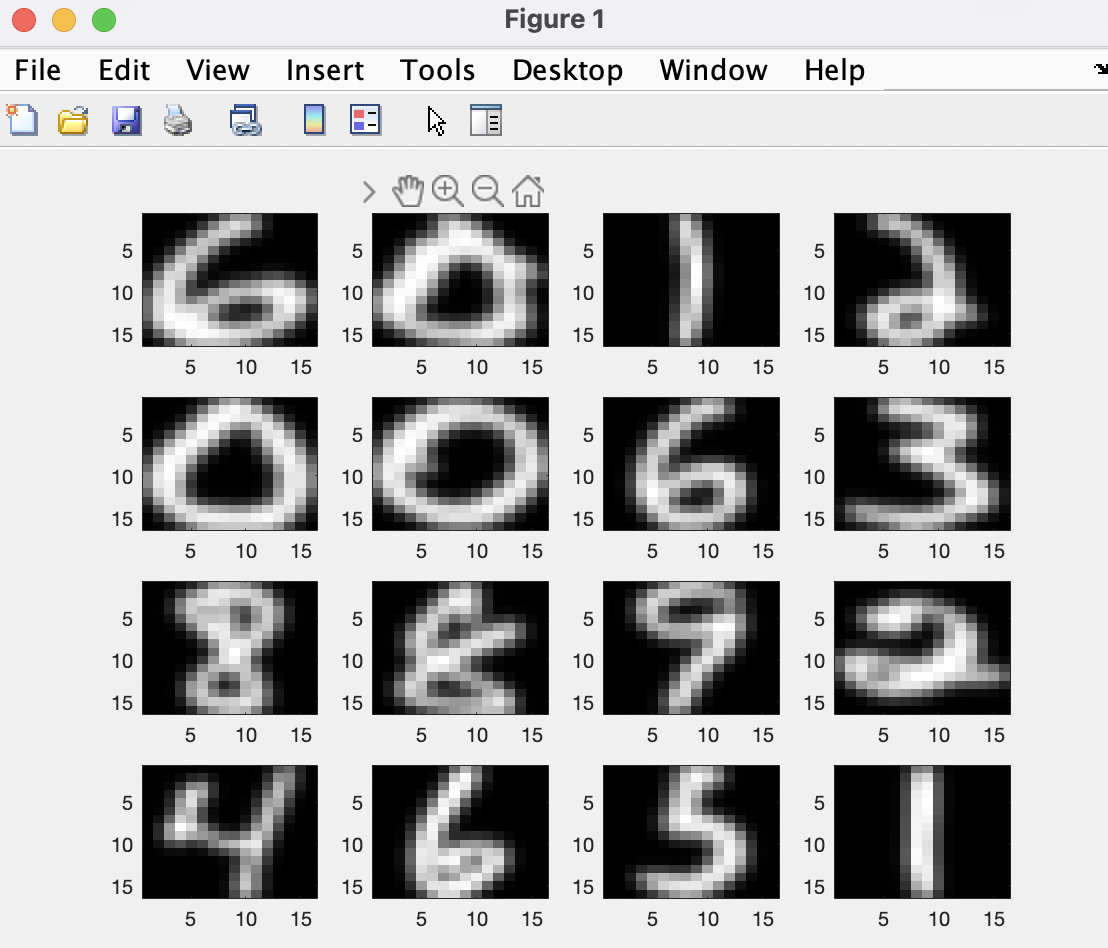
\includegraphics[scale=0.8]{Images/MAT 167 FPP Fig 1.png}

        \textit{Figure 1: The first 16 images of the training dataset put into image form}
    \end{center}

    \hskip 12pt From the image, we can see the first 16 columns of the training dataset visualized. Here, note that the images are split into 16 x 16 grids (leading to their mutation to 256 x 1 vectors), as well as the fact that we -as humans- can distinguish between the different numbers though they don't look exactly the same. 

    \vskip 06pt

    \hskip 12pt This ability to distinguish is exactly what we aim to replicate.

  \section{THE CENTROID CLASSIFICATION ALGORITHM}
    \label{SECT 03:THE CENTROID ALGORITHM}

      \hskip 12pt The centroid algorithm is a very basic, intuitive, and simple algorithm used to classify data in general. It's used often in terms of clustering and generally dictates that a data point is classified with the category it's closest to. In this case, we determine proximity between a data point and a category by comparing the euclidean distance between the point and the category mean (or the centroid).

      \subsection{DESCRIPTION OF THE ALGORITHM}
        \label{SUBSECT 3.1:CENTROID DESCRIPTION}

        \hskip 12pt The first step in the centroid algorithm is to determine the centroid, that is, the 256 mean pixel values for each digit from 0-9. To do this, we simply take a subset of the data and for a given digit (9 for example), we look into the training dataset -and the labels- and we subset the pixel color values for all images (column vectors) that represent the number 9.

        \vskip 06pt

        \hskip 12pt Next, we simply take the average value for each row. This makes sense because, if our training data is accurate, the pixels often included in the images representing 9 will be darker. So, the digit 9 will be shown clearer because weird images that aren't as representative of 9 will be dimmed down... simply put, their effect won't have a great effect on estimating the color values for the number 9. In essence, this is determining the centroid: the corresponding pixel values that generally correlate to a given number.

        \vskip 06pt

        \hskip 12pt When we do this for each number, we get the following images representing the centroids for each digit:

        \begin{center}
            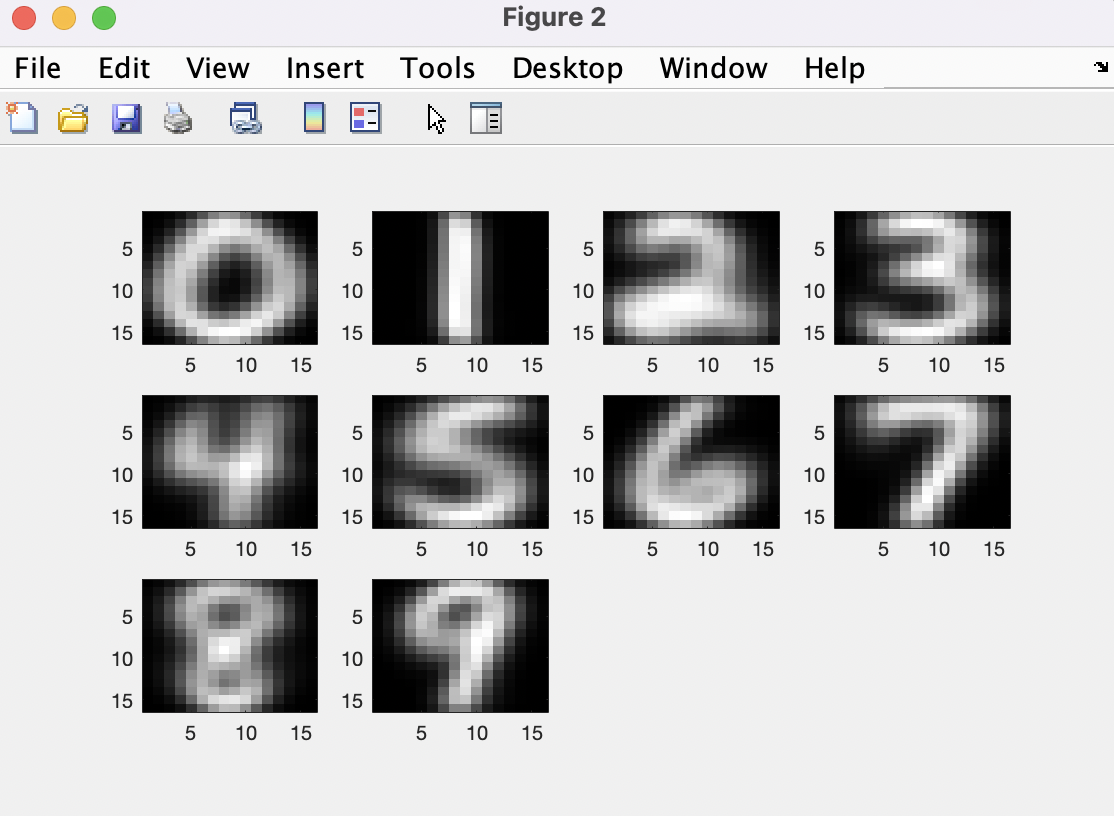
\includegraphics[scale=0.8]{Images/MAT 167 FPP Fig 2.png}
            
            \textit{Figure 2: Image depicting the centroids representing each digit, in image form. Note that when we average the values and find the centroid, it's clear to see that we have a pretty good approximation of what pixels correlate to each digit}
        \end{center}

        \vskip 06pt

        \hskip 12pt After we get the associated centroid vectors for a given digit, we move onto classification and look at unknown image vectors in the test dataset.

        \vskip 06pt

        \hskip 12pt Here, we use the 2-norm, euclidean distance, to measure how far a digit is away from a centroid. In essence, we take a vector, find the distance between each digit and the 10 centroids (euclidean distance between the vectors), and find the centroid that yielded the smallest distance. The centroid with the smallest distance is the one closest to a number and so, we classify that unknown image as the digit the centroid represents... We then do this for all 4649 image vectors in the test dataset.

        \vskip 06pt

        \hskip 12pt Then lastly, and pretty straightforwardly, we create a confusion matrix depicting our accuracy- where the rows are the true digits of the test sets and the columns are the counts of the digits that we classified. This will be shown clearer in the description of results.

        

      \subsection{DESCRIPTION OF THE RESULTS}
       \label{SUBSECT 3.2:CENTROID RESULTS}

          \begin{center}
              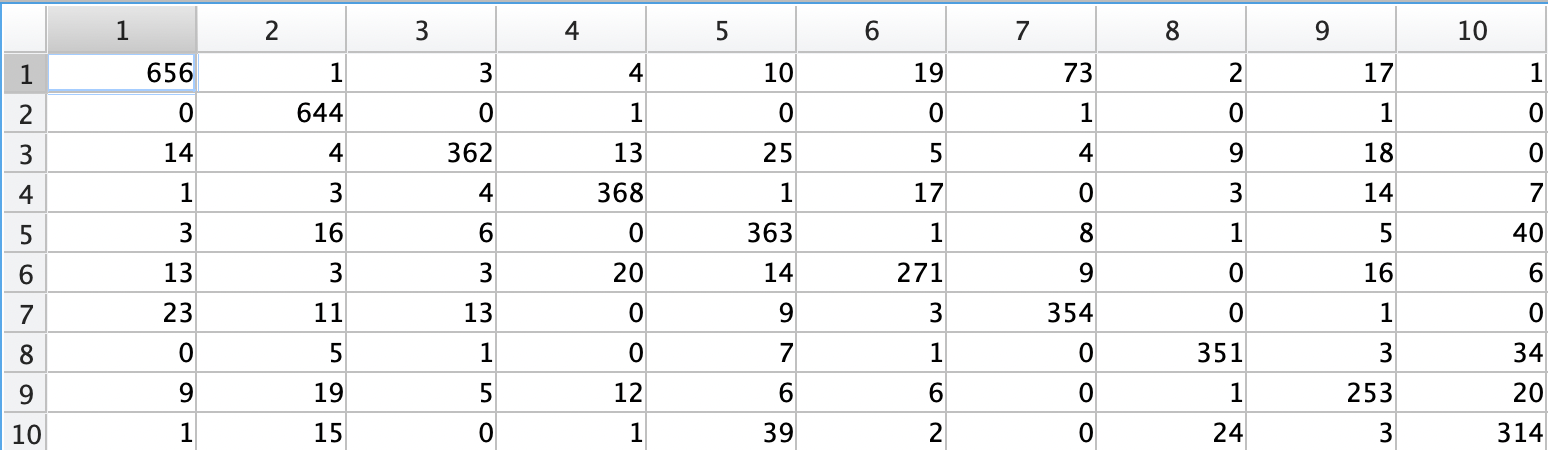
\includegraphics[scale = 0.65]{Images/MAT 167 FPP Fig 3.png}

              \textit{Figure 3: The confusion matrix associated with the centroid algorithm. This shows the accuracy of the algorithm where the values on the diagonal are counts of correctly classified images}
          \end{center}

          \vskip 06pt

          \hskip 12pt Here, we see clearer the confusion matrix. In essence, for each digit $k-1$ for $1\leq k \leq 10$, we find how many times that digit was properly guessed, how many times it was incorrectly guessed, and which values it was incorrectly guessed as.

          \vskip 06pt

          \hskip 12pt More broadly, the $k$ rows represent the true digit. So, the sum of row 1 would be the amount of times the image 0 was in the test dataset. The $j$ columns represent the amount of times the the digit was classified as our model as the $j-1$ digit. So, the first entry for (1,1) indicates that for images with the true value 0, they were classified correctly, as 0, 656 times. The next entry for (1,2) indicates that for images with the true value 0, 1 was classified incorrectly as 1. The entry (2,1) indicates that for values with the true value 1, none were classified incorrectly as 0.

          \vskip 06pt

          \hskip 12pt As the confusion matrix is understood better, one notes that the diagonal entries represent the amount of times a given digit was classified correctly, for that digit (within the row). 

          \vskip 06pt

          \hskip 12pt Overall, there were a few concerning instances where 20-80 images were classified incorrectly just as one different number (let alone classified incorrectly for the digit). Furthermore, 3936/4649 images were classified correctly: an accuracy rate of 0.84663368. However, the algorithm isn't bad in the sense that it still, very clearly, will classify an image more often than not. 

          \vskip 06pt

          \hskip 12pt Regardless, it begs the question that for instances where the classification needs to be very exact, can we get a higher accuracy?

      \section{THE SVD CLASSIFICATION ALGORITHM}
        \label{SECT 04:SVD CLASSIFICATION ALGORITHM}

        \vspace{06pt}

        \hskip 12pt The Singular Value Decomposition (SVD) is a powerful matrix factorization which factors a matrix A into three components such that
        
        \begin{center}
            $A = U \Sigma V^T$
        \end{center}

        where $U$ is an m x m orthonormal matrix containing the column vectors of the left singular vectors for $AA^T$, $\Sigma$ is an m x n diagonal matrix with non-negative real values called singular values which are the square roots of the eigenvalues for $AA^T$ or $A^TA$, and $V$ is an n x n orthonormal matrix containing the right singular vectors for $A^TA$.

        \vskip 06pt

        \hskip 12pt Broadly, the main essence of SVD in this case as that we can take the largest singular values which represent the "greatest direction" of the vectors. So, we can use SVD on matrix $A$ and take the most important singular values to filter out noise. Generally, the greatest singular vectors are most representative of the columns in matrix A. The smaller singular values correlate to singular vectors where the column vectors of A are represented by smaller, more variable coefficients in regard to those singular vectors. This algorithm is the difference between having one approximation for all images in a digit (centroid algorithm) vs having a different approximation for each image vector (SVD).

        \subsection{DESCRIPTION OF THE ALGORITHM}
          \label{SECT 04.01:SVD DESCRIPTION}

         \hskip 12pt To give a more in-depth explanation of SVD, we begin by noting that the SVD of $A$, as mentioned earlier, can be factored further. Specifically,

         \begin{center}
             $A = \sum^m_{i=1}\sigma_i\bs{u}_i\bs{v}_i^T$

             $\bs{a}_j = \sum^m_{i=1}(\sigma_iv_{ij})\bs{u}_i$
         \end{center}

        \hskip 12pt This tells us that the columns of $A$, or the distinct images, can actually be represented as coordinates of a vector in $U$. In other words, images can be approximated as linear combinations of the left singular vectors $\bs{u}_i$, which are orthogonal bases for a given digit. Thus, we move on to the first step.

        \vskip 06pt


        \hskip 12pt The first step is to pool the column vectors relating to a given digit. So, our matrix $A$ becomes a matrix of the column vectors correlating to a digit in the training set. From there, we do rank 17 SVD meaning that we take the top 17 singular values and vectors (and dismiss the remaining, less import, singular values / vectors that could provide unnecessary noise). Then, we take the $U$ orthonormal bases for each digit, yielding an array of size 256 x 17 x 10. This is essentially an array of 10 matrices that all contain the 17 $\bs{u}_i$ basis vectors in $\mathbb{R}^{256}$. Again, since each column vector is ultimately a vector in basis $U$, we don't need the singular values nor the right singular vectors. This is step A.

        \vskip 06pt

        \hskip 12pt In the next step, we compute the expansion coefficients for each image in the test dataset. Currently, we have, for a given digit, a 256 x 17 matrix containing the 17 $\bs{u_i}$ basis vectors. To calculate the expansion coefficients, we map each test image in the 256 x 4649 test dataset onto the vectors for a given digit (we get the inner product of the bases and the test images for a given digit). This yields a 17 x 4649 matrix for each digit and distinct expansion coefficients to approximate each different image vector onto the $U$ subspace.

        \vskip 06pt

        \hskip 12pt The beauty of this is that we can show each image vector as combinations of orthonormal base $U$ (then calculate Euclidean distance) while taking out the most important singular vectors- the most important information (parsing out noise that could distort our classification).
        
        \subsection{DESCRIPTION OF THE RESULTS}
          \label{SECT 04.02:SVD RESULTS}

        \hskip 12pt Next, we compute the approximations for each given digit, which is given by multiplying the 256 x 17 $U$ bases for a given digit against each coefficient vector in the 17 x 4649 coefficient matrix. This yields a 256 x 4649 matrix where each column vector is a unique approximation of the individual images against the digit $U$ base; this is done for each digit.

        \vskip 06pt

        \hskip 12pt With our approximations for each image, the remaining process is similar to that of the centroid algorithm. For a given image, we find the euclidean distance between that image vector and our 10 approximations (one for each digit). We use the euclidean distance as a metric to measure error primarily because it's the same metric used in the centroid algorithm and would thus make it easier to compare the algorithm. Furthermore, because we're using orthonormal basis vectors, the euclidean distance is an accurate measure (due to Pythagorean theorem). That is to say, we find the smallest $k$ that minimizes
        
        \begin{center}
            $\underset{min}{\alpha_i}||\bs{z}-\sum^k_{i=1}\alpha_i\bs{u}_i||_2$
        \end{center}
        
        \hskip 12pt Then, we label that image vector as the digit for which the euclidean distance was smallest. Then, just as before, we compute a confusion matrix.

        \begin{center}
            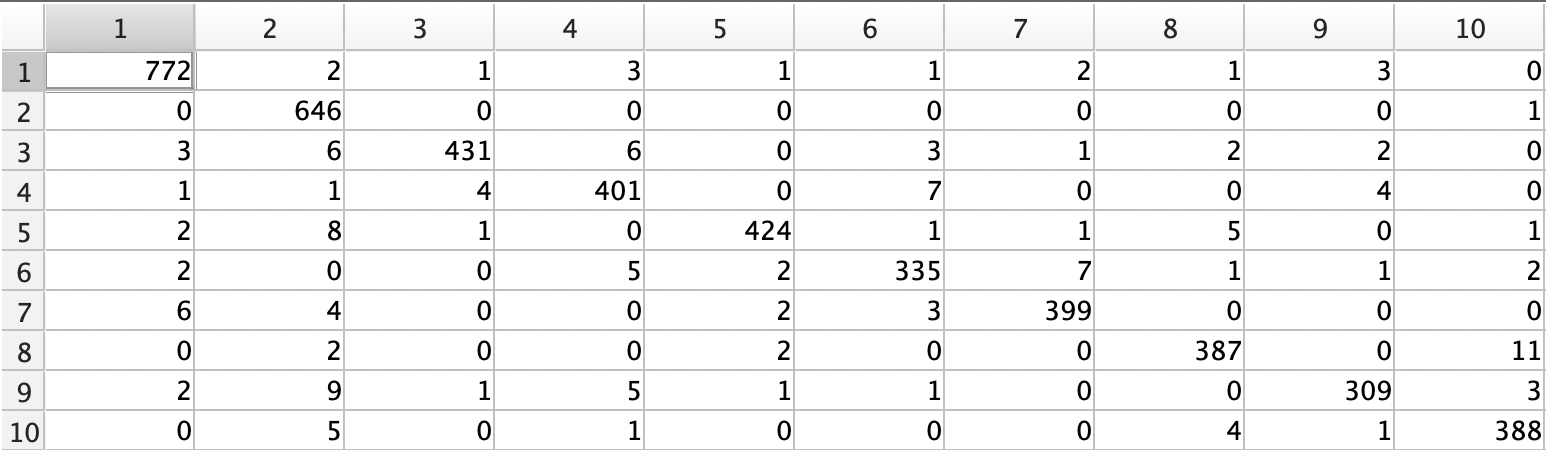
\includegraphics[scale = 0.65]{Images/MAT 167 FPP Fig 4.png}

            \textit{Figure4: The confusion matrix for the SVD algorithm; note that the results appear to be far more accurate than the centroid algorithm.}
        \end{center}

        \vskip 06pt

        \hskip 12pt The first thing immediately noticeable is that this confusion matrix appears more accurate overall. In total, it appears to have classified 4492/4649 images correctly: an accuracy rate of 0.9662293.

        \vskip 06pt

        \hskip 12pt Quite clearly, we see the superiority of SVD to the centroid algorithm because SVD is able to create an individual approximation specific to each image vector. Furthermore, we understand that not only does SVD create individual approximations per image but it also creates \textit{very accurate} approximations.

      \section{ANALYSIS}
        \label{SECT 05:ANALYSIS}

    \hskip 12pt Overall, the SVD algorithm is far more accurate than the centroid algorithm. We find the following accuracy for a given algorithm:

    \begin{center}
        \begin{tabular}{c|c|c}
            \hline
            Digit & Centroid & SVD \\
            \hline
            0 & 0.8346 & 0.9822 \\
            1 & 0.9954 & 0.9985 \\
            2 & 0.7974 & 0.9493 \\
            3 & 0.8804 & 0.9593 \\
            4 & 0.8194 & 0.9571 \\
            5 & 0.7634 & 0.9437 \\
            6 & 0.8551 & 0.9638 \\
            7 & 0.8731 & 0.9627 \\
            8 & 0.7644 & 0.9334 \\
            9 & 0.7870 & 0.9724 \\
        \end{tabular}
    \end{center}

    \vskip 06pt

    \hskip 12pt So, it's clear to see that for every digit, SVD proved noticeably superior and consistent with accurate not dropping below 0.93. The hardest digits to classify, it seems, are the digits 8 and 5 which yielded the lowest accuracy rates for SVD (0.9334 and 0.9437 respectively) and the centroid algorithm (0.7644 and 0.7634 respectively). On the other hand, the easiest digit to identify (by far) is the digit 1 with respective accuracies for the centroid and SVD algorithms as 0.9954 and 0.9985. One reason for these results could be because 1 is the easiest digit to draw and so, images will be less variable and more distinct from other digits. As for the letter 8, it's likely difficult because it could be easily confused for digits 0, 6, or 9 (all of which consist of distinct circles). In fact, both 8 and 5 were confused most often for 9 both in the centroid and SVD algorithm.

    \vskip 06pt

    \hskip 12pt Overall, SVD proves to be superior. In terms of overall accuracy, SVD (0.9662) classified digits more than 10 percentage points higher than the centroid algorithm (0.8466). Furthermore, for each digit, SVD was more accurate than the centroid algorithm. This difference in accuracy is the result of the difference between approximating a digit based on overall means vs distinct linear combinations for each image vector. However, this is just in terms of accuracy.

    \vskip 06pt

    \hskip 12pt In terms of speed, centroid is superior due to its simplicity; however, it'd be dependent on the situation to determine if the increase in speed makes up for the lack of accuracy (with small datasets though, this difference in speed is negligible). Furthermore, it'd be interesting to determine accuracy based on classifying the right number, or classifying numbers allowing for certain error. This would also be dependent on the situation but for simplicity in weighing algorithms, we determine accuracy as the proportion of correct classifications. In which case, SVD proves superior overall and stratified for each digit where its overall accuracy is about 12 percentage points higher than centroid and for each digit, accuracy was (on average) also more than 10 percentage points higher.

    \vspace*{12pt}

  \section{CONCLUSIONS}
    \label{SECT 06:CONCLUSIONS}


    \hskip 12pt As AI, as well as most electronics in general, get closer and closer to interacting more with the physical world, they require more physical inputs. One of these inputs is sight. In specific, a lot of problems today concern pattern recognition, where a machine needs to recognize and discern between visual inputs so it can respond appropriately. This exercise attempts to classify digits and test different algorithms to determine if one pattern recognition algorithm is better than another.

    \vskip 06pt 

    \hskip 12pt As part of the exercise, we use test and training data provided by the US Postal Service. Both test and training datasets contain 4649 images split by 16 x 16 grids and represented by 255 x 4649 matrices both. The primary difference is that the training dataset will be used to create approximations for what the digits should look like while the test datasets will be used to see how many we can classify properly (using the centroid and SVD algorithm). Otherwise, they're the same.

    \vskip 06pt

    \hskip 12pt The centroid algorithm consists of finding a vector that best represents a given digit by averaging the 255 pixel's color values among all the images of that given digit. Then, an unknown image is classified as a digit if the euclidean distance is smallest between the unknown image vector and that digit.

    \vskip 06pt

    \hskip 12pt For SVD, we similarly find approximations for the image vectors. However, in contrast with the centroid algorithm that finds one approximation for a given digit type, SVD finds an 10 approximations by digit, for \textit{each} image vector in the test dataset. Furthermore, we can take only the most import information for classification and parse out possible noise. This method relies on the Singular Value Decomposition and the fact that the training column space for a digit can be decomposed into the sum of the left singular value bases.

    \vskip 06pt

    \hskip 12pt In our analysis, we found that the hardest digits to identify were 8 and 5 while the easiest was 1. Regardless, however, although centroid would be faster due to simplicity, SVD proved far more accurate. In terms of overall accuracy and accuracy for each digit type, SVD was at least 10 percentage points more accurate (with the exception of the digit 1). 

    \vskip 06pt

    \hskip 12pt Overall, we conclude that SVD is generally superior to the centroid algorithm. The centroid algorithm is simple, easy-to-understand, and its accuracy wasn't bad; for large datasets where distinction is more obvious, it may even be preferred. However, SVD is overall far more accurate such that the complexity and increase in computing power is made up for in accuracy consistently over 93\%. Thus, we conclude, that SVD is preferable if there is computing power to support it.

  \section{COMPUTER PROGRAM}
    \label{SECT 07:COMPUTER PROGRAM}

      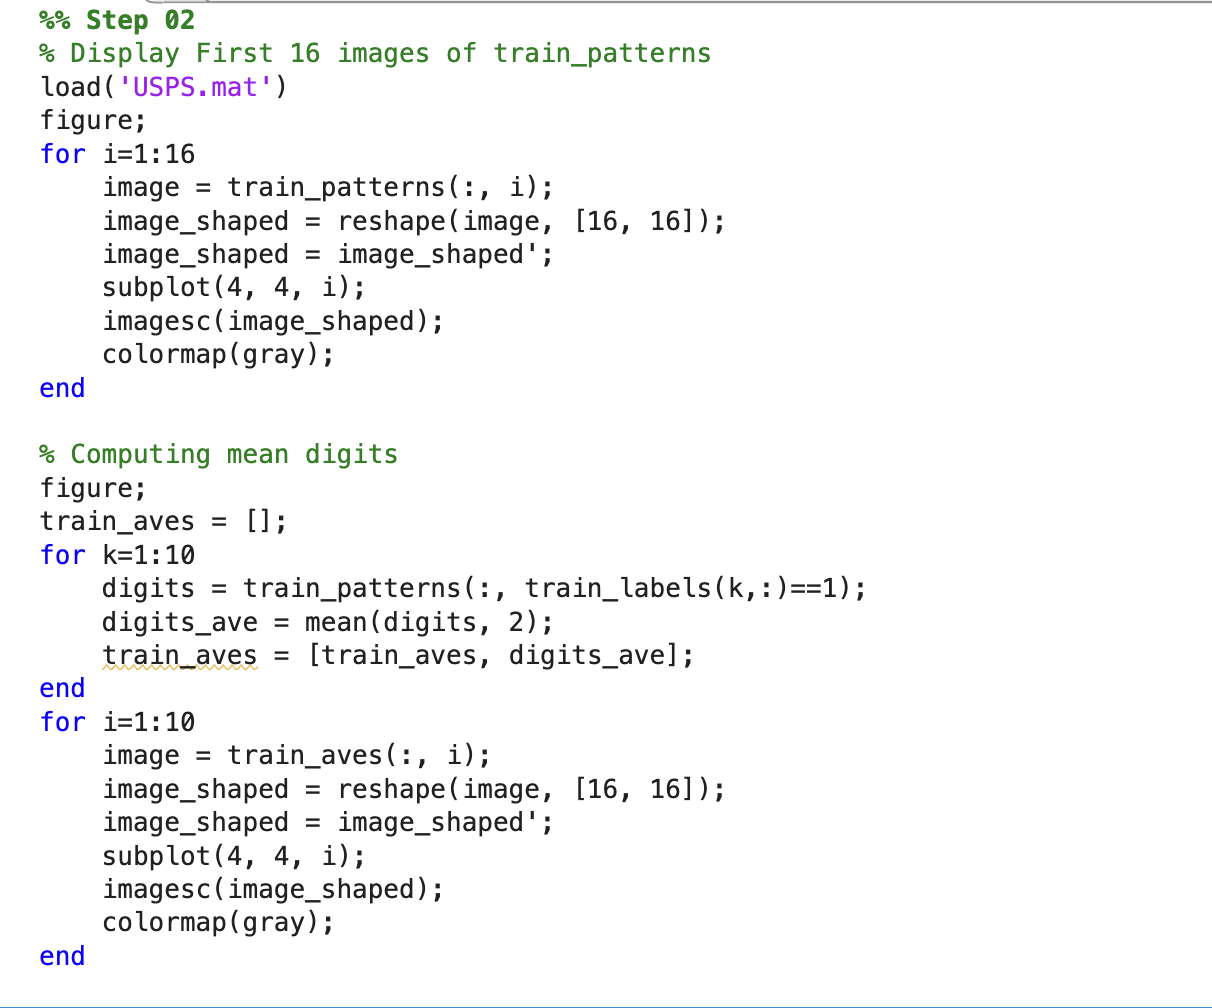
\includegraphics[scale = 0.8]{Images/MAT 167 FPP Code 1.png}

      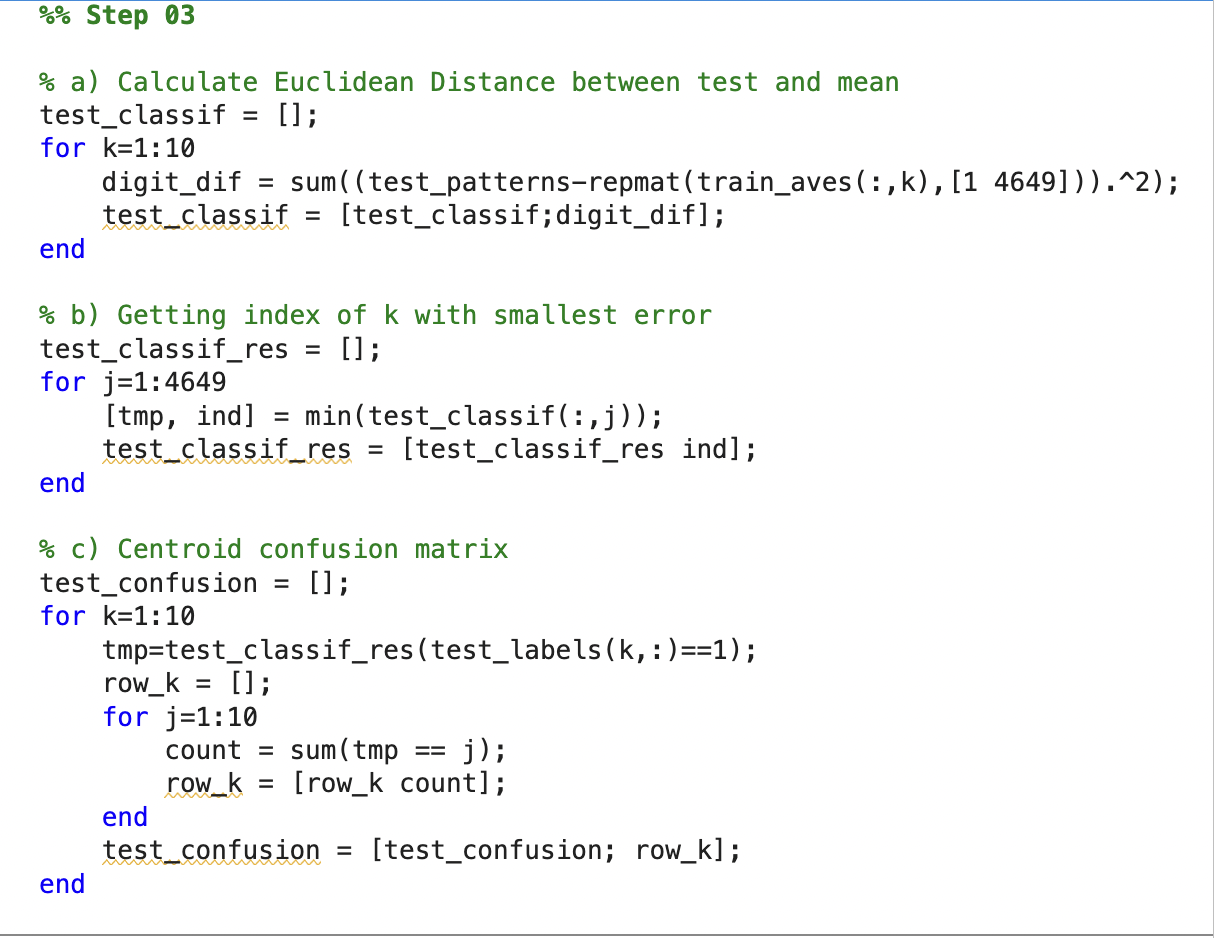
\includegraphics[scale = 0.7]{Images/MAT 167 FPP Code 2.png}

      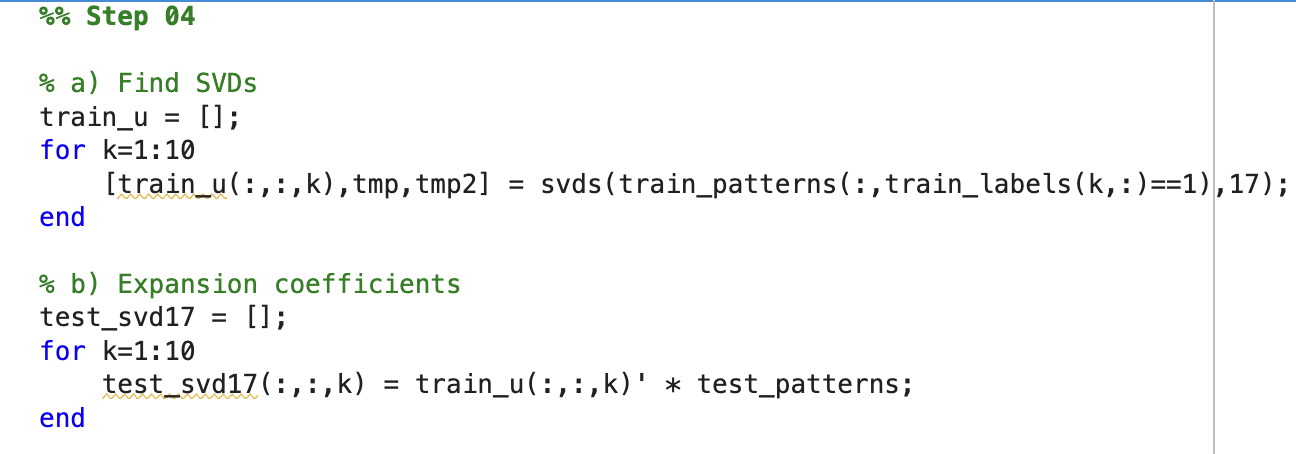
\includegraphics[scale = 0.7]{Images/MAT 167 FPP Code 3.png}

      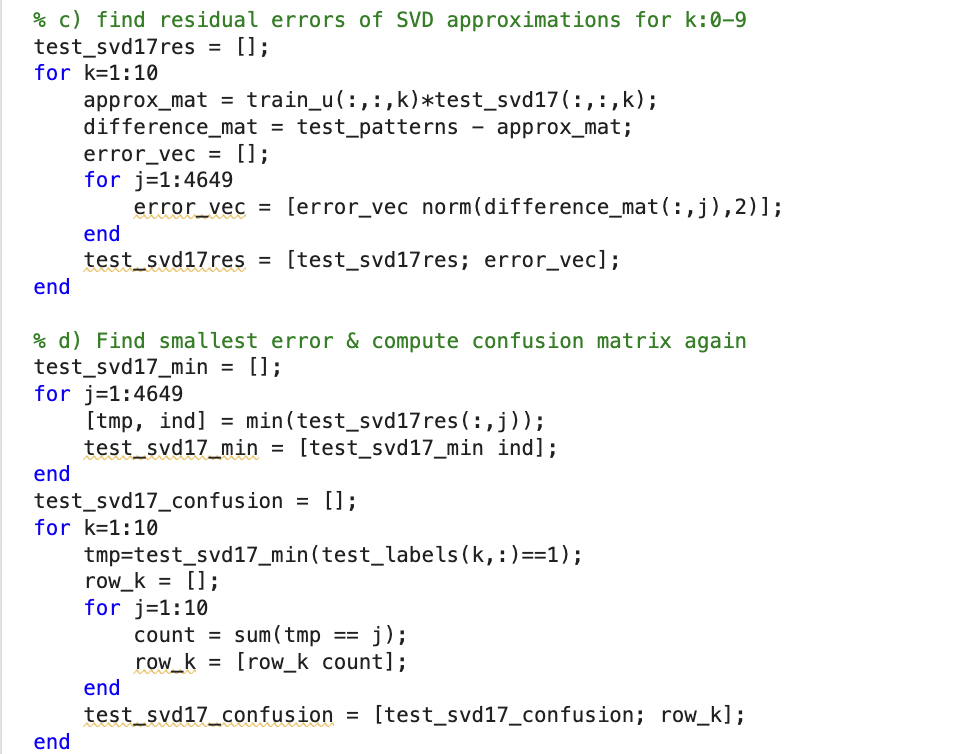
\includegraphics[scale = 0.8]{Images/MAT 167 FPP Code 4.png}


\end{document}
